\phantomsection
\section*{Manual de Usuario}
\addcontentsline{toc}{section}{Manual de Usuario}

Este manual proporciona una guía básica para el uso de la aplicación, explicando las funcionalidades disponibles y cómo acceder a ellas.

\subsection*{1. Inicio de la aplicaci\'on}
Al ejecutar la aplicación, se muestra una pantalla de inicio de sesión con opciones para iniciar sesión o registrarse.

\begin{figure}[H]
    \centering
    \includegraphics[width=0.6\textwidth]{images/manualDeUsuario/InicioAplicación.png}
    \caption*{Pantalla de inicio de sesión}
\end{figure}

\subsection*{2. Registro de un nuevo usuario}
Para crear una cuenta, el usuario debe seleccionar la opción \texttt{Register} y completar el formulario.

\begin{itemize}
    \item Introducir el número de teléfono, nombre de usuario y contraseña.
    \item Para modificar la imagen de perfil, introducir la url de la imagen deseada, y pulsar el botón de la derecha.
    \item Pulsar el botón \texttt{register}.
\end{itemize}

\begin{figure}[H]
    \centering
    \begin{minipage}[b]{0.48\textwidth}
        \centering
        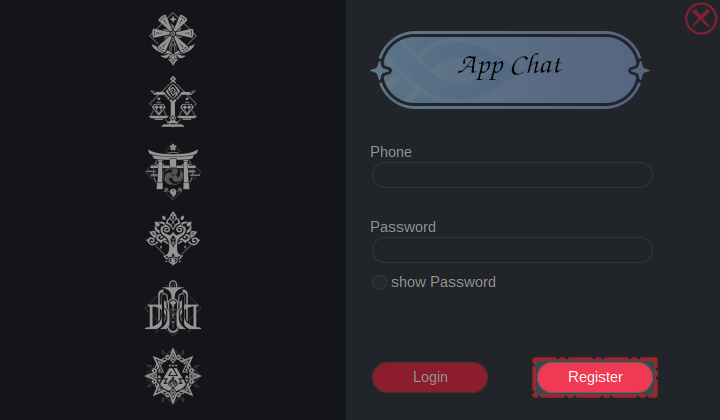
\includegraphics[width=\textwidth]{images/manualDeUsuario/registro1.png}
        \caption*{Formulario de registro - Parte 1}
    \end{minipage}
    \hfill
    \begin{minipage}[b]{0.48\textwidth}
        \centering
        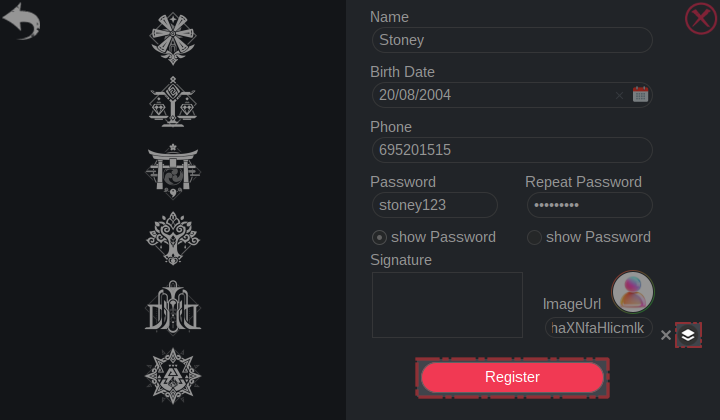
\includegraphics[width=\textwidth]{images/manualDeUsuario/registro2.png}
        \caption*{Formulario de registro - Parte 2}
    \end{minipage}
\end{figure}

\subsection*{3. Inicio de sesión}
Para iniciar sesión, el usuario debe introducir sus credenciales en la pantalla de inicio de sesión y pulsar el botón \texttt{Login}.

\begin{figure}[H]
    \centering
    \begin{minipage}[b]{0.48\textwidth}
        \centering
        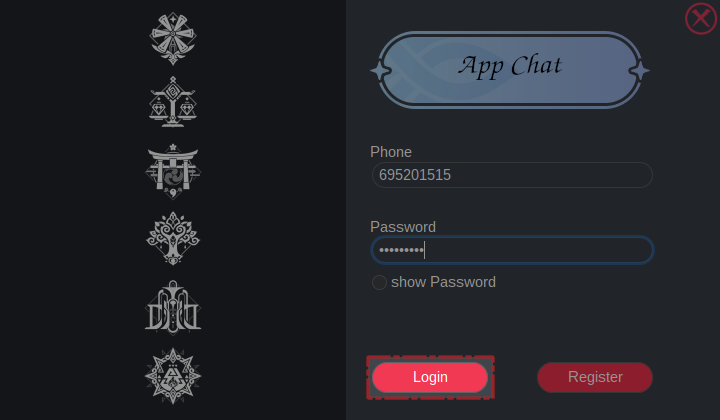
\includegraphics[width=0.96\textwidth]{images/manualDeUsuario/InicioSesion1.png}
        \caption*{Pantalla de inicio de sesión}
    \end{minipage}
    \hfill
    \begin{minipage}[b]{0.48\textwidth}
        \centering
        
\includegraphics[width=\textwidth]{images/manualDeUsuario/InicioSesion2.png}
        \caption*{Pantalla principal}
    \end{minipage}
\end{figure}

Tras iniciar sesión, el usuario accede a la pantalla principal de la aplicación, desde donde puede ver sus contactos y grupos, así como realizar otras operaciones.

\subsection*{4. Añadir un nuevo contacto}
Para añadir un nuevo contacto, el usuario debe pulsar el botón para acceder a la lista de contactos y luego seleccionar la opción \texttt{Add Contact}. 

\begin{figure}[H]
    \centering
    \begin{minipage}[b]{0.48\textwidth}
        \centering
        \includegraphics[width=\textwidth]{images/manualDeUsuario/AñadirContacto1.png}
        \caption*{Pantalla principal}
    \end{minipage}
    \hfill
    \begin{minipage}[b]{0.48\textwidth}
        \centering
        \includegraphics[width=\textwidth]{images/manualDeUsuario/AñadirContacto2.png}
        \caption*{Lista de usuarios}
    \end{minipage}
\end{figure}

A continuación, el usuario debe introducir el número de teléfono del contacto, el nombre que desea asignarle y pulsar el botón \texttt{Añadir}.

\begin{figure}[H]
    \centering
    \includegraphics[width=0.58\textwidth]{images/manualDeUsuario/AñadirContacto3.png}
    \caption*{Formulario para añadir contacto}
\end{figure}
